\subsection{3.7 Metallic bonding}
    \begin{minipage}{25mm}
        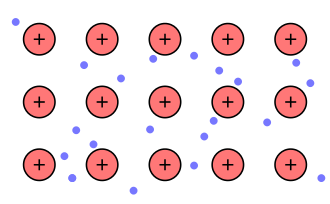
\includegraphics[width=2.5cm]{src/3_Chemical_bondings/images/Metallische Bindung.png}
    \end{minipage}
    \begin{minipage}{42mm}
        Positiv geladene Kerne umgeben von einer negativ geladenen Elektronenwolke. Metalle haben
        Defizit an VE $\rightarrow$ zu wenig VE, um Kovalente Bindung einzugehen. Frei bewegliche Ladungen 
        (Elektronenwolke) sind Ursache für gute Strom- und Wärmeleitfähigkeit.
    \end{minipage}